\achapter{3}{Metric Spaces} \label{sec:metric_spaces}


\vspace*{-17 pt}
\framebox{
\parbox{\dimexpr\linewidth-3\fboxsep-3\fboxrule}
{\begin{fqs}
\item What is a metric and what is a metric space? 
\item How are the Euclidean, taxicab, and max metric different and how are they similar?
\end{fqs}}}

\vspace*{13 pt}

\csection{Introduction}

Metric spaces are particular examples of topological spaces. A metric space is a space that has a metric defined on it. A metric is a function that measures the distance between points in a metric space. 

We are familiar with one special metric, the Euclidean metric $d_E$ in $\R^2$ where 
\[d_E((x_1,x_2),(y_1,y_2)) = \sqrt{(x_1-y_1)^2 + (x_2-y_2)^2}.\]
\begin{figure}[ht]
\begin{center}
\resizebox{!}{2.0in}{
\includegraphics{Euclidean_metric}}
\end{center}
\caption{The Euclidean distance between $(x_1,x_2)$ and $(y_1,y_2)$ and the Euclidean unit circle in $\R^2$.}
\label{F:Euclidean_metric}
\end{figure}
Using this metric, the distance between two points $(x_1,x_2)$ and $(y_1,y_2)$ is the length of the segment connecting the points, while the unit circle (the set of points a distance 1 from the origin) looks like what we think of as a circle as illustrated in Figure \ref{F:Euclidean_metric}.

As we will see, there are many other metrics that can be defined on $\R^n$, or on other sets. 

 
\begin{pa} Consider the function $d_T$ that assigns to each pair of points in $\R^2$ the real number 
\[d_T((x_1,x_2),(y_1,y_2)) = | x_1-y_1 | + | x_2-y_2 |.\] 
This function $d_T$ is sometimes called the \emph{taxicab metric}\index{metric!taxicab} or \emph{distance} because the distance between points $x$ and $y$ can be thought of as obtained by driving around a city block rather than going directly from point $x$ to point $y$. 

Any distance function should satisfy certain properties: the distance between two points should never be negative, the distance from point $A$ to point $B$ should be the same as the distance from point $B$ to point $A$, the shortest distance between two points $A$ and $B$ should never be more than the distance from $A$ to some point $C$ plus the distance from $C$ to $B$, and the distance between points should only be zero if the points are the same. In this activity, we determine if $d_T$ has these properties. Let $x=(x_1,x_2)$ and $y=(y_1,y_2)$ in $\R^2$. 

\be
\item Prove that $d_T(x,y) \geq 0$. 

\item Prove that $d_T(x,y) = d_T(y,x)$. 

\item  Prove that $d_T(x,y) = 0$ if and only if $x = y$. 

\item Let $z = (z_1,z_2)$ in $\R^2$. Read the proof of Lemma \ref{lem:abs_TI} (below) and then use Lemma \ref{lem:abs_TI} to show that 
\[d_T(x,y) \leq d_T(x,z) + d_T(z,y).\]	
(Do you have any questions about the proof of the lemma?)

\begin{lemma} \label{lem:abs_TI} Let $a$ and $b$ be real numbers. Then
\[| a+b | \leq | a | + | b |.\]
\end{lemma}

\begin{proof} Let $a$ and $b$ be real numbers. To prove the lemma we consider cases. 
\begin{description}
\item[Case 1: $a \geq 0$ and $b \geq 0$.] In this case $a+b$ is nonnegative and so $| a | = a$, $| b | = b$, and $| a+b | = a+b$. Then
\[| a+b | = a+b =  | a | + | b |.\]
\item[Case 2: $a \leq 0$ and $b \leq 0$.] In this case $a = -a'$ and $b = -b'$ where $a'$ and $b'$ are nonnegative. It follows from Case 1 that 
\[| a+b | = | -(a'+b') | = | a'+b' | = a'+b' = | a' | + | b' | = | -a' | + | -b' | = | a | + | b |.\]
\item[Case 3: One of $a$ or $b$ is positive and the other negative.] Without loss of generality we assume $a > 0$ and $b < 0$. Again we consider cases. Note that $b < 0$ implies $a+b < a$. 
	\begin{itemize}
	\item Suppose $b \geq -2a$. Then $a+b \geq -a$ and so $-a \leq a+b < a$. It follows that  
\[| a+b | \leq a = | a | < | a | + | b |.\]  
	\item The last case is when $b < -2a$. In this case $-b > 2a$ and so 
	\[| b | = -b > 2a = 2| a | > | a |.\]
	 Then $a+b < a = | a | < | b |$. Finally, $a > 0$ implies $a+b > b = -| b |$. So
\[- | b | < a+b < | b |\]
and 
\[| a+b | \leq | b | < | a | + | b |.\]
	\end{itemize}
\end{description}
This proves our lemma for every possible pair $a$, $b$.
\end{proof}  

\item A picture to illustrate the taxicab distance $d_T$ between (points $x_1,x_2)$ and $(y_1,y_2)$ is shown in Figure \ref{F:PA_metric}. Draw a picture of the unit circle (the set of points a distance 1 from the origin) using the Taxicab metric. Explain your reasoning.
\begin{figure}[ht]
\begin{center}
\resizebox{!}{2.0in}{
\includegraphics{Taxicab}}
\end{center}
\caption{The taxicab distance between $(x_1,x_2)$ and $(y_1,y_2)$ in $\R^2$.}
\label{F:PA_metric}
\end{figure}

	
\ee


\end{pa}

\begin{comment}

\ActivitySolution

\be
\item Since $| a | \geq 0$ for any $a \in \R$, we have that $| x_1-y_1 | \geq 0$ and $| x_2-y_2 | \geq 0$. Thus,
\[d_T(x,y) = | x_1-y_1 | + | x_2-y_2 | \geq 0.\]

\item  Since $| -1 | = 1$, we have that 
\begin{align*}
d_T(x,y) &= | x_1-y_1 | + | x_2-y_2 | \\
	&= | (-1)(y_1-x_1) | + | (-1)(y_2-x_2) | \\
	&= | (-1) | | y_1-x_1 | + | (-1) | | y_2-x_2 | \\
	&= | y_1-x_1 | + | y_2-x_2 | \\
	&= d_T(y,x).
\end{align*}


\item  Suppose 
\[d_T(x,y) =  | x_1-y_1 | + | x_2-y_2 | = 0.\]
Since $|a| \geq 0$ for every real number $a$, it follows that 
\[| x_1-y_1 | = 0 = | x_2-y_2 |.\]
Therefore, $x_1=y_1$ and $x_2=y_2$, which makes $x = y$. 

Now suppose $x = y$. Then $x_1=y_1$ and $x_2=y_2$ and 
\[| x_1-y_1 | = 0 = | x_2-y_2 |.\]
it follows that   
\[d_T(x,y) = | x_1-y_1 | + | x_2-y_2 | = 0+0 = 0.\]  

\item   First note that 
\begin{align*}
d(x,z) + d(z,y) &= \left(| x_1-z_1 | + | x_2-z_2 | \right) + \left( | z_1-y_1 | +  | z_2-y_2 | \right) \\
	&= \left(| x_1-z_1 | + | z_1-y_1 | \right) + \left( | x_2-z_2 |  + | z_2-y_2 | \right).
\end{align*}
Applying Lemma \ref{lem:abs_TI} give us 
\begin{align*}
d(x,z) + d(z,y) &= \left( | x_1-z_1 | + | z_1-y_1 | \right) + \left(| x_2-z_2 |  + | z_2-y_2 | \right) \\
	&\geq \left(| (x_1-z_1) + (z_1-y_1) | \right) + \left(| (x_2-z_2) + (z_2-y_2) | \right) \\
	&= | x_1-y_1 | + | x_2-y_2 | \\
	&= d(x,y).
\end{align*}

\item A point $(x_1,x_2)$ will be a distance 1 from the origin if $|x_1| + |x_2| = 1$. This will only happen if 
\[|x_2| = 1- |x_1| \text{ and } -1 \leq x_1, x_2 \leq 1.\]
In other words, the point $(x_1,x_2)$ must lie on one of the lines 
\begin{align*}
x_2 &= 1-x_1 \text{ if } x_1, x_2 \geq 0 \\
x_2 &= 1+x_1 \text{ if } x_1<0 \text{ and } x_2 \geq 0 \\
x_2 &= -1+x_1 \text{ if } x_1\geq 0 \text{ and } x_2 < 0 \\
x_2 &= -1-x_1 \text{ if } x_1, x_2 \leq 0.
\end{align*}
So the unit circle using the metric $d_T$ in $\R^2$ looks as depicted in Figure \ref{F:taxicab_circle}.
\begin{figure}[ht]
\begin{center}
\resizebox{!}{2.0in}{\includegraphics{Taxicab_circle}}
\end{center}
\caption{The unit circle in $\R^2$ using the taxicab metric.}
\label{F:taxicab_circle}
\end{figure}
	
\ee


\end{comment}

The taxicab metric can be extended to $\R^n$ for any $n \geq 1$ as follows. If $x = (x_1, x_2, \ldots, x_n)$ and $y = (y_1, y_2, \ldots, y_n)$ are in $\R^n$, then the taxicab distance $d_T(x,y)$ from $x$ to $y$ is defined as
\[d_T(x,y) = |x_1-y_1| + |x_2-y_2| + \cdots + |x_n-y_n| = \sum_{i=1}^n |x_i-y_i|.\]


\csection{Metric Spaces}

For most of our mathematical careers our mathematics has taken place in $\R^2$, where we measure the distance between points $(x_1,x_2)$ and $(y_1,y_2)$ with the standard Euclidean distance $d_E$. In our preview activity we saw that the function $d_T$ satisfies many of the same properties as $d_E$. These properties allow us to use $d_E$ or $d_T$ as distance functions. We call any distance function a \emph{metric}, and any space on which a metric is defined is called a \emph{metric space}. 

\begin{definition} A \textbf{metric}\index{metric} on a space $X$ is a function $d : X \times X \to \R^+ \cup \{0\}$ that satisfies the properties: 
\begin{enumerate}
\item $d(x,y) \geq 0$ for all $x,y \in X$,
\item $d(x,y) = 0$ if and only if $x = y$ in $X$,
\item $d(x,y) = d(y,x)$ for all $x, y \in X$, and
\item $d(x,y) \leq d(x,z) + d(z,y)$ for all $x,y,z \in X$.
\end{enumerate}
\end{definition}

Properties 1 and 2 of a metric say that a metric is \emph{positive definite}, while property 3 states that a metric is \emph{symmetric}. Property 4 of the definition is usually the most difficult property to verify for a metric and is called the \emph{triangle inequality}\index{triangle inequality}. 

\begin{definition} A \textbf{metric space}\index{metric space} is a pair $(X,d)$, where $d$ is a metric on the space $X$. 
\end{definition}

When the metric is clear from the context, we just refer to $X$ as the metric space.


\begin{activity} \label{act:MS_metrics} For each of the following, determine if $(X,d)$ is a metric space. If $(X,d)$ is a metric space, explain why. If $(X,d)$ is not a metric space, determine which properties of a metric $d$ satisfies and which it does not. If $(X,d)$ is a metric space, give a geometric description of the unit circle (the set of all points in $X$ a distance $1$ from the zero element) in the space.  
	\ba
	\item $X = \R$, $d(x,y) = \max\{|x|,|y|\}$. 

	
	\item $X = \R$, $d(x,y) = \begin{cases} 0 & \text{ if } x=y \\ 1 & \text{ if } x \neq y. \end{cases}$


	\item $X = \R^2$, $d((x_1,x_2),(y_1,y_2)) = \max\{| x_1-y_1 |, | x_2-y_2 | \}$ 

 
	\item $X = C[0,1]$, the set of all continuous functions on the interval $[0,1]$, 
	\[d(f,g) = \ds \int_0^1 | f(x) - g(x) | \, dx.\] 

	\ea

\end{activity}

\begin{comment}

\ActivitySolution

	\ba
	\item  This function $d$ is not a metric on $\R$. It is the case by definition that $d(x,y) \geq 0$ for all $x,y \in \R$. If $x \neq y$, then at least one of $x,y$ is not 0 and $d(x,y) > 0$. Also, $d(1,1) = 1$, not 0, so $d$ does not satisfy the second property of a metric. This $d$ is symmetric, and also satisfies the triangle inequality. To see why the triangle inequality is satisfied, let $x,y,z \in \R$. We look at two cases. 
\begin{itemize}
\item If $|x| \geq |z|$, then 
\[d(x,z)=|x| \text { and } d(x,y)+d(y,z) \geq |x| + d(y,z) \geq |x| = d(x,z).\]
\item If $|x| < |z|$, then 
\[d(x,z)=|z| \text { and } d(x,y)+d(y,z) \geq d(x,y) + |z| \geq |z| = d(x,z).\]
\end{itemize}
In either case,
\[d(x,z) \leq d(x,y)+d(y,z)\]
and $d$ satisfies the triangle inequality.
	
	\item This $d$ does define a metric on $X$. By definition, $d(x,y) \geq 0$ for all $x, y \in X$. If $x \neq y$, then $y \neq x$, so $d$ is symmetric. By definition, $d(x,y) = 0$ if and only if $x=y$. Let $x,y,z \in X$. Then 
$d(x,y)+d(x,z) = 0$ if and only if $x = y = z$. In this case
\[0 = d(x,z) = 0 + 0 = d(x,y) = d(y,z).\]
If $x$, $y$, and $z$ are not all equal, then 
\[d(x,y) + d(y,z) \geq 1 \geq d(x,z).\]
So $d$ satisfies the triangle inequality and $d$ is a metric. Note that this argument did not depend on the elements of $X$, so this $d$ defines a metric on any set. It is interesting to notice that the unit circle in this metric is all of $\R$ except for the origin. 

	\item Let $x = (x_1,x_2)$ and $y = (y_1, y_2)$. Now $|a| \geq 0$ for any real number $a$, so $d(x,y) \geq 0$. That $d$ is symmetric follows from the fact that $|-a| = |a|$ for any real number $a$:
	\[d(x,y) =\max\{ | x_1 - y_1 |, | x_2 - y_2 | \} = \max\{| y_1 - x_1 |, | y_2 - x_2 |\} = d(y,x).\]
If $x = y$, then 
\[d(x,y) =\max\{ | x_1 - y_1 |, | x_2 - y_2 | \} = \max\{0,0\} = 0.\]
If $d(x,y) = 0$, then
\[0 = 	\max\{ | x_1 - y_1 |, | x_2 - y_2 | \}.\]
But if $x_1 \neq y_1$ or $x_2 \neq y_2$, then $|x_1-y_1| > 0$ or $|x_2 - y_2 | > 0$, forcing $d(x,y) > 0$. So if $d(x,y) = 0$, then $x = y$. 

Now we consider the triangle inequality. Let $x = (x_1,x_2)$, $y=(y_1, y_2)$, $z = (z_1, z_2)$ in $\R^2$. We know that 
\[|x_1-z_1| = |(x_1-y_1) + (y_1-z_1)| \leq |x_1-y_1| + |y_1-z_1|\]
and
\[|x_2-z_2| = |(x_2-y_2) + (y_2-z_2)| \leq |x_2-y_2| + |y_2-z_2|.\]

It is the case that $d(x,z) = \max\{|x_1-z_1|,|x_2-z_2|\}$ is either equal to $|x_1-z_1|$ or $|x_2-z_2|$. Suppose that $d(x,z) = |x_1-z_1|$. Then 
\[d(x,z) \leq |x_1-y_1| + |y_1-z_1| \leq \max\{|x_1-y_1|, |x_2-y_2|\} + \max\{|y_1-z_1|, |y_2-z_2|\} = d(x,y) + d(y,z).\]
Similarly, if $d(x,z) = |x_2-z_2|$. Then 
\[d(x,z) \leq |x_2-y_2| + |y_2-z_2| \leq \max\{|x_1-y_1|, |x_2-y_2|\} + \max\{|y_1-z_1|, |y_2-z_2|\} = d(x,y) + d(y,z).\]
So $d$ satisfies the triangle inequality. Thus, $d$ is a metric on $X$. This metric is called the \emph{max} metric. In this case, the unit circle is the set of points $(x_1,x_2)$ such that $\max\{|x_1|, |x_2|\} = 1$. This is the set of points $(x_1,x_2)$ where $x_1 = 1$ and $-1 \leq x_2 \leq 1$ or $x_2 = 1$ and $-1 \leq x_1 \leq 1$. In other words, the unit circle in this space is the square centered at the origin of side length 2. 

	\item We show that $d$ is a metric. Let $f, g$ be in $C[0,1]$. If we integrate a nonnegative function over any interval, the resulting area is never negative. So $d(f,g) \geq 0$. Since $|a - b| = |b - a|$ for any real numbers $a$ and $b$, it follows that $d$ is symmetric. From calculus we know that 
	\[d(f,f) = \int_0^1 |f(x)-f(x)| \, dx = \int_0^1 0 \, dx = 0.\]
	Now suppose that $d(f,g) = 0$. To show that $f = g$, we proceed by contradiction and assume that $f \neq g$. So there exists $c \in [0,1]$ such that $f(c) \neq g(x)$. Since $f$ and $g$ are continuous, there must be some small interval $I$ in $[0,1]$ containing $c$ such that $f(x) \neq g(x)$ on $I$. Then ${f(x) - g(x)} > 0$ on $I$ and 
	\[\int_I |f(x) - g(x)| \, dx > 0.\]
Therefore,	
	\[d(f,g) = \int_0^1 |f(x)-g(x)| \, dx = \int_{x \notin I} |f(x)-g(x)| \, dx + \int_{x \in I} |f(x)-g(x)| \, dx > 0.\]
So $d(f,g) = 0$ implies that $f=g$. 

Finally, we consider the triangle inequality. Let $h \in C[0,1]$. Then
\begin{align*}
\int_0^1 |f(x)-g(x)| \, dx &= \int_0^1 |(f(x)-h(x))+(h(x)-g(x)| \, dx \\
	&\leq \int_0^1 |f(x)-h(x)| + |h(x)-g(x)| \, dx \\
	&= \int_0^1 |f(x)-h(x)| \, dx + \int_0^1 |h(x)-g(x)| \, dx \\
	&= d(f,h) + d(h,g).
\end{align*}	 

The unit circle is difficult to visualize here, but it is the set of functions $f$ that bound one unit of area between the graph of $f$ and the $x$-axis on $[0,1]$. 
	\ea

\end{comment}


It should be noted that not all metric spaces are infinite. We discuss one metric on a finite space in the following example.

\begin{example} \label{exp:finite_ms} Let $X = \{a,b,c\}$ and define $d: A \times A \to \R^+ \cup \{0\}$ with the entries in Table \ref{T:finite_metric_ex}.
\begin{table}[ht]
\begin{center}
\begin{tabular}{c|ccc}
	&$a$ 	&$b$		&$c$ \\ \hline
$a$	&$0$		&$3$		&$5$ \\ 
$b$	&$3$		&$0$		&$4$ \\
$c$	&$5$		&$4$		&$0$ 
\end{tabular}
\caption{Table of values for a function $d$.}
\label{T:finite_metric_ex}
\end{center}
\end{table}
By definition we have $d(x,y) \geq 0$ for all $x, y \in X$ with $d(x,y) = 0$ if and only if $x=y$. Since the table is symmetric around the diagonal, we can see that $d(x,y) = d(y,x)$ for all $x,y \in X$. The only item to verify is the triangle inequality. If $d(x,y) = 0$, then
\[d(x,y) = 0 \leq d(x,z) + d(z,y)\]
for any $x,y \in X$. If $d(x,z) = 0$, then $x=z$ and 
\[d(x,y) = d(z,y) \leq d(z,z) + d(z,y).\]
That leaves three cases to consider, when $x$, $y$, and $z$ are distinct. Now 
\begin{align*}
d(a,b) &= 3 \leq 5+4 = d(a,c) + d(c,b), \\
d(a,c) &= 5 \leq 3+4 = d(a,b) + d(b,c), \\
d(b,c) &= 4 \leq 3+5 = d(b,a) + d(a,c).
\end{align*}
So $d$ is a metric on $X$. 
\end{example}

Example \ref{exp:finite_ms} shows that even finite sets can be metric spaces. In fact, we can make a finite metric space by taking any finite subset $S$ of a metric space $(X,d)$ and use as a metric the restriction of $d$ to $S$. Example \ref{exp:finite_ms} illustrates this by letting $a = (0,0)$, $b = (3,0)$, and $c = (3,4)$ in $\R^2$. Then $d$ is the restriction of the Euclidean metric to the set $X$. Another way to construct a finite metric space is to start with a finite set of points and make a graph with the points as vertices. Construct edges so that the graph is connected (that is, there is a path from any one vertex to any other) and give weights to the edges as illustrated in Figure \ref{F:Graph_metric}. We then define a metric $d$ on $S$ by letting $d(x,y)$ be the length of a shortest path between vertices $x$ and $y$ in the graph. For example, $d(b,c) = d(b,e) + d(e,c) = 9$ in this example. 
\begin{figure}[h]
\begin{center}
\resizebox{!}{2.0in}{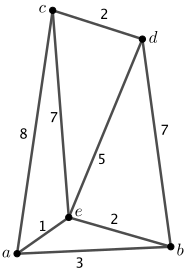
\includegraphics{Graph_metric.eps}}
\caption{A graph to define a metric.} 
\label{F:Graph_metric}
\end{center}
\end{figure}
%\includegraphics[trim=left bottom right top, clip]{file}

Just as with the Euclidean and taxicab metrics, item (c) in Activity \ref{act:MS_metrics} can be extended to $\R^n$ as follows. If $x = (x_1, x_2, \ldots, x_n)$ and $y = (y_1, y_2, \ldots, y_n)$ are in $\R^n$, then the maximum distance $d_M(x,y)$ from $x$ to $y$ is defined as
\[d_M(x,y) = \max\{| x_1-y_1 |, | x_2-y_2 |, |x_3-y_3|, \ldots, |x_n-y_n| \} = \max_{1 \leq i \leq n} \{|x_i-y_i|\}.\]
The metric $d_M$ is called the \emph{max} metric{\index{metric!max}. In the following section we prove that the Euclidean metric is in fact a metric. Proofs that $d_T$ and $d_M$ are metrics are left to Exercises (\ref{ex:Taxicab}) and (\ref{ex:Max}). 

\csection{The Euclidean Metric on $\R^n$}
The metric space that is most familiar to us is the metric space $(\R^2, d_E)$, where 
\[d_E((x_1,x_2), (y_1,y_2)) = \sqrt{(x_1-y_1)^2 + (x_2-y_2)^2}\] 
The metric $d_E$ called the \emph{standard} or \emph{Euclidean}\index{metric!Euclidean} metric on $\R^2$. 

We can generalize this Euclidean metric from $\R^2$ to any dimensional real space. Let $n$ be a positive integer and let $x = (x_1, x_2, \ldots, x_n)$ and $y = (y_1, y_2, \ldots, y_n)$ be in $\R^n$. We define $d_E : \R^n \times \R^n \to \R$ by 
\[d_E(x,y) = \sqrt{(x_1-y_1)^2 + (x_2-y_2)^2 + \cdots (x_n-y_n)^2} = \sqrt{\sum_{i=1}^n (x_i-y_i)^2}.\]
In the next activity we will show that $d_E$ satisfies the first three properties of a metric.  

\begin{activity} Let $x = (x_1, x_2, \ldots, x_n)$ and $y = (y_1, y_2, \ldots, y_n)$ be in $\R^n$.
\ba
\item Show that $d_E(x,y) \geq 0$. 

\item Show that $d_E(x,y) = d_E(y,x)$.

\item Show that if $x=y$, then $d_E(x,y) = 0$.

\item Show that if $d_E(x,y) = 0$, then $x=y$. 

\ea

\end{activity}

\begin{comment}

\ActivitySolution

\ba
\item Since $(x_i-y_i)^2 \geq 0$ for each $i$, we have 
\[d_E(x,y) =  \sqrt{\sum_{i=1}^n (x_i-y_i)^2} \geq 0.\] 

\item Since $(x_i-y_i)^2 = (y_i-x_i)^2$ for each $i$, we have 
\[d_E(x,y) =  \sqrt{\sum_{i=1}^n (x_i-y_i)^2} = \sqrt{\sum_{i=1}^n (y_i-x_i)^2} = d_E(y,x).\] 

\item If $x = y$, then $x_i = y_i$ and $x_i-y_i = 0$ for each $i$ . Then
\[d_E(x,y) =  \sqrt{\sum_{i=1}^n (x_i-y_i)^2} =  \sqrt{\sum_{i=1}^n 0} = 0.\] 

\item Suppose $d_E(x,y) = 0$. If $x_k \neq y_k$ for some $k$, then $(x_k - y_k)^2 > 0$. This makes
\[d_E(x,y) =  \sqrt{\sum_{i=1}^n (x_i-y_i)^2} =  \sqrt{\sum_{i \neq k} (x_i-y_i)^2 + (x_k-y_k)^2} \geq \sqrt{0 +  (x_k-y_k)^2} > 0.\]
So we must have $x_i = y_i$ for every $i$ and $x=y$. 

\ea

\end{comment}

Proving that the triangle inequality is satisfied is often the most difficult part of proving that a function is a metric. We will work through this proof with the help of the Cauchy-Schwarz Inequality. 

\begin{lemma}[Cauchy-Schwarz Inequality\index{Cauchy-Schwarz Inequality}] \label{lem:CS_Euclidean} Let $n$ be a positive integer and $x = (x_1, x_2, \ldots, x_n)$, $y=(y_1, y_2, \ldots, y_n)$ be in $\R^n$. Then 
\begin{equation} \label{eq:SL}
\sum_{i=1}^n x_iy_i \leq  \left(\sqrt{\sum_{i=1}^n x_i^2}\right) \left(\sqrt{\sum_{i=1}^n y_i^2}\right).
\end{equation} 
\end{lemma}

\begin{activity} Before we prove the Cauchy-Schwarz Inequality, let us analyze it in two specific situations.
	\ba
	\item Let $x=(1,4)$ and $y = (3,2)$ in $\R^2$. Verify the Cauchy-Schwarz Inequality in this case.

	\item Let $x=(1,2, -3)$ and $y = (-4, 0, -1)$ in $\R^3$. Verify the Cauchy-Schwarz Inequality in this case.

	\ea
\end{activity}

\begin{comment}

\ActivitySolution
	\ba
	\item Here we have 
	\[\sum_{i=1}^2 x_iy_i = (1)(3) + (4)(2) = 11\]
	and
	\[\left(\sqrt{\sum_{i=1}^2 x_i^2}\right) \left(\sqrt{\sum_{i=1}^2 y_i^2}\right) = \sqrt{1+9}\sqrt{16+4} = \sqrt{200} \approx 14.1.\]

	\item Here we have 
	\[\sum_{i=1}^3 x_iy_i = (1)(-4) + (2)(0) + (-3)(-1) = -1\]
	and
	\[\left(\sqrt{\sum_{i=1}^3 x_i^2}\right) \left(\sqrt{\sum_{i=1}^3 y_i^2}\right) = \sqrt{1+4+9}\sqrt{16+0+1} = \sqrt{238} \approx 15.4.\]

	\ea

\end{comment}

Now we prove the Cauchy-Schwarz Inequality.

\begin{proof}[Proof of the Cauchy-Schwarz Inequality]  Let $n$ be a positive integer and $x = (x_1, x_2, \ldots, x_n)$, $y=(y_1, y_2, \ldots, y_n)$ be in $\R^n$. To verify (\ref{eq:SL}) it suffices to show that 
\[\left(\sum_{i=1}^n x_iy_i\right)^2 \leq  \left(\sum_{i=1}^n x_i^2\right) \left(\sum_{i=1}^n y_i^2\right).\]
This is difficult to do directly, but there is a nice trick one can use.
Consider the expression
\[\sum (x_i-\lambda y_i)^2.\]
(All of our sums are understood to be from 1 to $n$, so we will omit the limits on the sums for the remainder of the proof.) Now
\begin{align}
0 & \leq \sum (x_i-\lambda y_i)^2 \notag \\
	&= \sum \left(x_i^2 - 2\lambda x_iy_i + \lambda^2 y_i^2 \right) \notag \\
	&= \left( \sum y_i^2 \right)\lambda^2 - 2\left(\sum x_iy_i\right) \lambda + \left(\sum x_i^2\right). \label{eq:SL_1}
\end{align}
To interpret this last expression more clearly, let $a=\sum y_i^2$, $b=-2\sum x_iy_i$ and $c = \sum x_i^2$. The inequality defined by (\ref{eq:SL_1}) can then be written in the form
\[p(\lambda) = a \lambda^2 + b \lambda + c \geq 0.\]
So we have a quadratic $p(\lambda)$ that is never negative. This implies that the quadratic $p(\lambda)$ can have at most one real zero. The quadratic formula gives the roots of $p(\lambda)$ 
as
\[\frac{-b \pm \sqrt{b^2-4ac}}{2a}.\]
If $b^2-4ac > 0$, then $p(\lambda)$ has two real roots. Therefore, in order for $p(\lambda)$ to have at most one real zero we must have
\[0 \geq b^2-4ac = 4 \left(\sum x_iy_i\right)^2 - 4\left(\sum y_i^2\right)\left(\sum x_i^2\right)\]
or
\[\left(\sum y_i^2\right)\left(\sum x_i^2\right) \geq \left(\sum x_iy_i\right)^2.\]
This establishes the Cauchy-Schwarz Inequality.
\end{proof}

One consequence of the Cauchy-Schwarz Inequality that we will need to show that $d_E$ is a metric is the following.

\begin{corollary} \label{cor:SL} Let $n$ be a positive integer and $x = (x_1, x_2, \ldots, x_n)$, $y=(y_1, y_2, \ldots, y_n)$ be in $\R^n$. Then 
\[\sqrt{\sum_{i=1}^n (x_i+y_i)^2} \leq \sqrt{\sum_{i=1}^n x_i^2} + \sqrt{\sum_{i=1}^n y_i^2}.\]
\end{corollary}

\begin{activity} Before we prove the corollary, let us analyze it in two specific situations.
	\ba
	\item Let $x=(1,4)$ and $y = (3,2)$ in $\R^2$. Verify Corollary \ref{cor:SL} in this case.
 
	\item Let $x=(1,2, -3)$ and $y = (-4, 0, -1)$ in $\R^3$. Verify Corollary \ref{cor:SL} in this case.

	\ea
\end{activity}

\begin{comment}

\ActivitySolution

	\ba
	\item Here we have 
	\[\sqrt{\sum_{i=1}^2 (x_i+y_i)^2} = \sqrt{4^2+6^2} = \sqrt{52} \approx 7.2\]
	and
	\[\sqrt{\sum_{i=1}^2 x_i^2} + \sqrt{\sum_{i=1}^2 y_i^2} = \sqrt{1+16} + \sqrt{9+4} = \sqrt{17}+\sqrt{13} \approx 7.7.\] 
 
	\item Here we have 
	\[\sqrt{\sum_{i=1}^3 (x_i+y_i)^2} = \sqrt{(-3)^1+2^2+(-4)^2} = \sqrt{29} \approx 5.4\]
	and
	\[\sqrt{\sum_{i=1}^3 x_i^2} + \sqrt{\sum_{i=1}^3 y_i^2} = \sqrt{1+4+9} + \sqrt{16+0+1} = \sqrt{14}+\sqrt{17} \approx 7.8.\] 


	\ea
	
\end{comment}

Now we prove Corollary \ref{cor:SL}.

\begin{proof}[Proof of Corollary \ref{cor:SL}] Let $n$ be a positive integer and $x = (x_1, x_2, \ldots, x_n)$, $y=(y_1, y_2, \ldots, y_n)$ be in $\R^n$. Now
\begin{align*}
\sum \left(x_i+y_i\right)^2 &= \sum \left(x_i^2 +2x_iy_i + y_i^2 \right) \\
	&= \sum x_i^2 + 2\sum x_iy_i + \sum y_i^2 \\
	&\leq \sum x_i^2 + 2\left(\sqrt{\sum x_i^2}\right) \left(\sqrt{\sum y_i^2} \right) + \sum y_i^2 \\
	&= \left(\sqrt{\sum x_i^2} + \sqrt{\sum y_i^2}\right)^2.
\end{align*}
Taking the square roots of both sides yields the desired inequality.
\end{proof}

We can now complete the proof that $d_E$ is a metric.

\begin{activity} Let $n$ be a positive integer and $x = (x_1, x_2, \ldots, x_n)$, $y=(y_1, y_2, \ldots, y_n)$, and $z=(z_1, z_2, \ldots, z_n)$ be in $\R^n$. Use Corollary \ref{cor:SL} to show that 
\[d_E(x,y) \leq d_E(x,z)+d_E(z,y).\]

\end{activity}

\begin{comment}

\ActivitySolution Now we can apply Corollary \ref{cor:SL} to verify that $d_E$ satisfies the triangle inequality.  Let $n$ be a positive integer and $x = (x_1, x_2, \ldots, x_n)$, $y=(y_1, y_2, \ldots, y_n)$ be in $\R^n$. Then
\begin{align*}
d_E(x,z) + d_E(z,y) &= \sqrt{\sum (x_i-z_i)^2} + \sqrt{\sum (z_i-y_i)^2} \\
	&\geq \sqrt{ \sum \left[(x_i-z_i)+(z_i-y_i)\right]^2}  \\
	&= \sqrt{ \sum (x_i-y_i)^2}  \\
	&= d_E(x,y).
\end{align*}

\end{comment}


This concludes our proof that the Euclidean metric is in fact a metric. 

We have seen several metrics in this section, some of which are given special names. Let $x = (x_1, x_2, \ldots, x_n)$ and $y = (y_1, y_2, \ldots, y_n)$
\begin{itemize}
\item The Euclidean metric $d_E$, where
\[d_E(x,y) = \sqrt{(x_1-y_1)^2 + (x_2-y_2)^2 + \cdots (x_n-y_n)^2} = \sqrt{\sum_{i=1}^n (x_i-y_i)^2}.\]
\item The Taxicab metric $d_T$, where 
\[d_T(x,y) = |x_1-y_1| + |x_2-y_2| + \cdots + |x_n-y_n| = \sum_{i=1}^n \{|x_i-y_i|\}.\]
\item The max metric $d_M$, where 
\[d_M(x,y) = \max\{| x_1-y_1 |, | x_2-y_2 |, |x_3-y_3|, \ldots, |x_n-y_n| \} = \max_{1 \leq i \leq n} \{|x_i-y_i|\}.\]
\end{itemize}
We have only shown that $d_T$ and $d_M$ are metrics on $\R^2$, but similar arguments apply in $\R^n$. Proofs are left to Exercises (\ref{ex:Taxicab}) and (
\ref{ex:Max}). In addition, the \emph{discrete metric}\index{metric!discrete}
\[d(x,y) = \begin{cases} 0 & \text{ if } x=y \\ 1 & \text{ if } x \neq y \end{cases}\]
makes any set $X$ into a metric space. The proof is left to Exercise (\ref{ex:MS_discrete}).

\csection{Summary}
Important ideas that we discussed in this section include the following.
\begin{itemize}
\item A metric on a space $X$ is a function that measures distance between elements in the space. More formally, a metric on a space $X$ is a function $d: X \times X \to \R^+ \cup \{0\}$ such that 
	\begin{enumerate}
	\item $d(x,y) \geq 0$ for all $x,y \in X$,
	\item $d(x,y) = 0$ if and only if $x = y$ in $X$,
	\item $d(x,y) = d(y,x)$ for all $x, y \in X$, and
	\item $d(x,y) \leq d(x,z) + d(z,y)$ for all $x,y,z \in X$.
	\end{enumerate}
A metric space is any space combined with a metric defined on that space.

\item The Euclidean, taxicab, and max metric are all metrics on $\R^n$, so they all provide ways to measure distances between points in $\R^n$. These metric are different in how they define the distances. 

	\begin{itemize}
	\item The Euclidean metric is the standard metric that we have used through our mathematical careers. For elements $x = (x_1, x_2, \ldots, x_n)$ and $y = (y_1, y_2, \ldots, y_n)$ in $\R^n$, the Euclidean metric $d_E$ is defined as
\[d_E(x,y) =  \sqrt{(x_1-y_1)^2 + (x_2-y_2)^2 + \cdots (x_n-y_n)^2} = \sqrt{\sum_{i=1}^n (x_i-y_i)^2}.\]
With this metric, the unit circle in $\R^2$ (the set of points a distance $1$ from the origin) is the standard unit circle we know from Euclidean geometry. 

	\item The taxicab metric $d_T$ is defined as
\[d_T(x,y) = |x_1-y_1| + |x_2-y_2| + \cdots + |x_n-y_n| = \sum_{i=1}^n |x_i-y_i|.\]
The unit circle in $\R^2$ using the taxicab metric is the square with vertices $(1,0)$, $(0,1)$, $(-1,0)$, and $(0,-1)$ when viewed in Euclidean geometry. 

	\item The max metric $d_M$ is defined by 
\[d_M(x,y) = \max\{| x_1-y_1 |, | x_2-y_2 |, |x_3-y_3|, \ldots, |x_n-y_n| \} = \max_{1 \leq i \leq n} \{|x_i-y_i|\}.\]
Under the max metric, the unit circle in $\R^2$ is the square with vertices $(1,1)$, $(-1,1)$, $(-1,-1)$, and $(1,-1)$ when viewed in Euclidean geometry.

	\end{itemize}
	
\end{itemize}


\csection{Exercises}

\be

\item \label{ex:MS_discrete} Let $X$ be a set.  Show that the function $d$ (the discrete metric) defined by 
\[d(x,y) = \begin{cases} 0 & \text{ if } x=y \\ 1 & \text{ if } x \neq y \end{cases}\]
is a metric. 

\begin{comment}

\ExerciseSolution Let $x$, $y$, and $z$ be in $X$. By definition, $d(x,y) \geq 0$, $d(x,y) = 0$ if and only if $x=y$, and $d(x,y) = d(y,x)$. So the only item to prove is the triangle inequality. We consider the cases $x \neq y$ and $x = y$. 
\begin{itemize}
\item If $x \neq y$, then 
\[d(x,y) + d(y,z) \geq 1 \geq d(x,z).\]
\item If $x=y$, then 
\[d(x,y) + d(y,z) = d(y,z) = d(x,z).\]
\end{itemize}
We conclude that $d$ is a metric on any set. 

\end{comment}


\item \label{ex:MS_mod_metric} Let $X = \{1,3,5\} \subset \Z$ and define $d: X \times X \to \R$ by $d(x,y) = xy - 1 \pmod{n}$. That is, $d(x,y)$ is the remainder when $xy - 1$ is divided by $n$. 
	\begin{itemize}
	\item For each value of $n$, determine if $d$ defines a metric on $X$. Prove your answers. 
	\item The unit circle in $\R^2$ with metric $d$ is the set of all points in $\R^2$ whose distance from the origin is $1$. If we let the distance be less than $1$, then we have what we call an open ball. We can make this same definition in any metric space.
	
\begin{definition} \label{def:ms_open_ball} Let $(Y, d_Y)$ be a metric space.  For any positive real number $r$, the \textbf{open ball centered at}\index{open ball in a metric space} $b$ \textbf{of radius} $r$ in $(Y, d_Y)$ is the  the set 
\[B(b,r) = \{y \in Y \mid d_Y(y,b) < r\}.\]
\end{definition}

If $(X,d)$ is a metric space for a given value of $n$, determine all of the open balls in $X$ centered at $1$. If $(X,d)$ is not a metric space, explain why. 
	\end{itemize}

\ba
\item $n = 4$

\item $n = 8$

\ea

\begin{comment}

\ExerciseSolution

\ba
\item  Since $xy-1 \pmod{4}$ is never negative, we see that $d(x,y) \geq 0$ for all $x,y \in X$. To determine if $d(x,y) = 0$ if and only if $x=y$, we calculate all of the distances as shown in Table \ref{T:d_example_4}.
\begin{table}[h]
\begin{center}
\begin{tabular}{|c|c|c|c|} \hline
		&$1$	&$3$	&$5$	\\ \hline
$1$		&$0$	&$2$	&$0$	\\ \hline
$3$		&$2$	&$0$	&$2$	\\ \hline
$5$		&$0$	&$2$	&$0$	\\ \hline
\end{tabular}
\caption{Values of $d$ with $n=4$.}
\label{T:d_example_4}
\end{center}	
\end{table}
Note that $d(1,5)=0$, but $1 \neq 5$. Thus, $d$ is not a metric on $X$. 

\item  Since $xy-1 \pmod{8}$ is never negative, we see that $d(x,y) \geq 0$ for all $x,y \in X$. To verify that $d(x,y) = 0$ if and only if $x=y$, we calculate all of the distances as shown in Table \ref{T:d_example_8}.
\begin{table}[h]
\begin{center}
\begin{tabular}{|c|c|c|c|} \hline
		&$1$	&$3$	&$5$	\\ \hline
$1$	&$0$	&$2$	&$4$	\\ \hline
$3$	&$2$	&$0$	&$6$	\\ \hline
$5$	&$4$	&$6$	&$0$	\\ \hline
\end{tabular}
\caption{Values of $d$ with $n=8$.}
\label{T:d_example_8}
\end{center}	
\end{table}
The symmetry along the main diagonal in Table \ref{T:d_example_8} also shows that $d(x,y) = d(y,x)$ for all $x, y \in X$. 

Finally, we consider the triangle inequality. Let $a,b,c \in X$. If $a=b$, then 
\[d(a,b) = 0 \leq d(a,c) + d(c,b).\]
So we only need consider the cases where $a \neq b$. Assume $a \neq b$. If $c = a$, then 
\[d(a,b) = d(c,b) = d(a,c) + d(c,b).\]
A similar result holds if $c = b$. So the only case left to consider is if $a$, $b$, and $c$ are all distinct. In this case, $d(a,b) \leq 6$, while $d(a,c) + d(c,b) \geq 2 + 4 = 6$. So 
\[d(a,b) \leq 6 \leq 2 + 4 \leq d(a,c) + d(c,b).\]
Therefore, $d$ is a metric on $X$ and $(X,d)$ is a metric space. 


The open balls centered at $a=1$ in $X$ are 
\begin{align*}
B(1,r) &= \{1\} \text{ if } r \leq 2, \\
B(1,r) &= \{1,3\} \text{ if } 2 < r \leq 4, \\
B(1,r) &= \{1,3,5\} \text{ if } 4 < r. 
\end{align*}

\ea

\end{comment}


\item \label{ex:MS_Q_metric} Let $Q$ be the set of all rational numbers in reduced form. A rational number $\frac{r}{s}$ is in reduced form if $s > 0$ and $r$ and $s$ have no common factors larger than $1$. Define $d : Q \times Q \to \R$ by 
\[d\left(\frac{a}{b}, \frac{r}{s}\right) = \max\{| a-r |, | b-s |\}.\]
	\ba
	\item Prove that $d$ is a metric. 
	
	\item A metric allows us to determine which elements in our metric space are ''close" together. Describe the set of elements in $Q$ that are a distance no more than $1$ from $\frac{2}{3}$ using this metric $d$. In other words, describe the open ball centered at $\frac{2}{3}$ with radius $1$ (see Definition \ref{def:ms_open_ball}).
	
	\item If $a$, $b$, and $c$ are elements of a metric space $(X, d_X)$, we say that $b$ is between $a$ and $c$ if $d_X(a,c) = d_X(a,b) + d_X(b,c)$. Using the Euclidean metric on $\Q$, there are infinitely many different rational numbers between $0$ and $1$ (the rational numbers between $0$ and $1$ that lie on the Euclidean line through $0$ and $1$. Describe all of the points in $(\Q,d)$ that are between $0$ and $1$.  
	
	\ea

\begin{comment}

\ExerciseSolution

	\ba
	\item Let $\frac{a}{b}$ and $\frac{r}{s}$ be rational numbers in reduced form. By definition we have that $d\left(\frac{a}{b}, \frac{r}{s}\right) \geq 0$. Since $|r-a| = |a-r|$ and $|s-b| = |b-s$, it follows that 
	\[d\left(\frac{a}{b}, \frac{r}{s}\right) =  \max\{| a-r |, | b-s |\} =  \max\{| r-a |, | s-b |\} = d\left(\frac{r}{s}, \frac{a}{b}\right).\]
	So $d$ is symmetric. 
	
	Suppose $d\left(\frac{a}{b}, \frac{r}{s}\right) = 0$. Then $\max\{| a-r |, | b-s |\} = 0$ which implies that both $|a-r| = 0$ and $|b-s| = 0$. From this we have that $a=r$ and $b=s$, or $\frac{a}{b} = \frac{r}{s}$. Conversely, suppose $\frac{a}{b} = \frac{r}{s}$. The fact that $\frac{a}{b} = \frac{r}{s}$ means that $as = br$. Since $a$ and $b$ share no prime factors, every prime in the prime factorization of $b$ must be a factor of $s$. Thus, $s = \pm b$. But since $b$ and $s$ are positive, it follows that $b=s$.  Cancelling $b$ from both sides of $as = br$ yields $a=r$. But this means that $|a-r| = |b-s| = 0$ and so $d\left(\frac{a}{b}, \frac{r}{s}\right) = 0$.
	
Lastly, we must verify the triangle inequality. Let $\frac{e}{f}$ be another rational number in reduced form. By the triangle inequality of the Euclidean metric, we know that 
\[|a - e| \leq |a-r| + |r-e| \text{ and }  |b-f| \leq |b-s| + |s-f|.\]
Now 
\[d\left(\frac{a}{b}, \frac{r}{s}\right) =  \max\{| a-r |, | b-s |\} \geq |a-r| \text{ and } d\left(\frac{a}{b}, \frac{r}{s}\right) =  \max\{| a-r |, | b-s |\} \geq |b-s|\]
and
\[d\left(\frac{r}{s}, \frac{e}{f}\right) =  \max\{| r-e |, | s-f |\} \geq |r-e| \text{ and } d\left(\frac{r}{s}, \frac{e}{f}\right) =  \max\{| r-e |, | s-f |\} \geq |s-f|.\]
So 
\[d\left(\frac{a}{b}, \frac{r}{s}\right) + d\left(\frac{r}{s}, \frac{e}{f}\right) \geq |a-r| + |r-e| \geq |a-e|\]
and
\[d\left(\frac{a}{b}, \frac{r}{s}\right) + d\left(\frac{r}{s}, \frac{e}{f}\right) \geq |s-d| + |s-f| \geq |b-f|.\]
Therefore,
\[d\left(\frac{a}{b}, \frac{r}{s}\right) + d\left(\frac{r}{s}, \frac{e}{f}\right) \geq \max\{|a-e|, |b-f|\} = d\left(\frac{a}{b}, \frac{e}{f}\right).\]
We conclude that $d$ is a metric. 
		
	\item An element $\frac{a}{b}$ in $Q$ is within $\frac{1}{2}$ of $\frac{2}{3}$ if
	\[d\left(\frac{a}{b}, \frac{2}{3}\right) \leq 1.\]
	This happens when
	\[\max\{|a-2|, |b-3|\} \leq 1.\]
We must then have $|a-2| \leq 1$ and $|b-3| \leq 1$. Now $|a-2| \leq 1$ when $1 \leq a \leq 3$ and $|b-3| \leq 1$ when $2 \leq b \leq 4$.  But $a$ and $b$ must be integers so $a$ can be $1$, $2$, or $3$ and $b$ can be $2$, $3$, or $4$. But it must also be the case that $a$ and $b$ have no common positive factors other than $1$, so the elements in $Q$ that are no more than a distance $1$ from $\frac{2}{3}$ are $\frac{1}{2}$, $\frac{1}{3}$, $\frac{1}{4}$, $\frac{2}{3}$, $\frac{3}{2}$, and $\frac{3}{4}$. 

\item Since $0 = \frac{0}{1}$ and $1 = \frac{1}{1}$ we have that $d(0,1) = 1$. So if $b = \frac{u}{v}$ is between $0$ and $1$, then 
\[1 = d(0,b) + d(b,1).\]
Now $d(0,b) = \max\{|u|, |v-1|\}$ and $d(1,b) = \max\{|u-1|, |v-1|\}$. We consider the cases. 
\begin{itemize}
\item Suppose $d(0,b) = |u|$ and $d(a,b) = |u-1|$. Then 
\[1 = |u| + |u-1|.\]
Since $u$ is an integer, the cases are $|u| = 0$ and $|u-1| = 1$, or $|u|=1$ and $|u-1| = 0$. When $u=0$, $b=0$.  When $|u-1|=0$ we have $u = 1$. The fact that  $|u-1| \geq |v-1|$ implies that $0 \geq |v-1|$ and $v = 1$. In this case $b = 1$. 

\item Suppose $d(0,b) = |u|$ and $d(a,b) = |v-1|$. Then 
\[1 = |u| + |v-1|.\]
The cases are $|u|=0$ and $|v-1| = 1$, or $|u| = 1$ and $|v-1| = 0$.  When $u=0$, $b=0$. When $|v-1| = 0$ we must have $v = 1$. The fact that $0 = |v-1| \geq |u-1|$ implies that $u=1$. 

\item Suppose $d(0,b) = |v-1|$ and $d(a,b) = |u-1|$. Then 
\[1 = |v-1| + |u-1|.\]
The cases are $|u-1|=0$ and $|v-1| = 1$, or $|u-1| = 1$ and $|v-1| = 0$.  When $|u-1|=0$ we have $u=1$. The fact that $0 = |u-1| \geq |v-1|$ tells us that $v=1$. So $b=1$. When $|v-1| = 0$, then $v=1$. The fact that  $0 = |v-1| \geq |u|$ implies that $u=0$. This makes $b=0$. 

\item Suppose $d(0,b) = |v-1|$ and $d(a,b) = |v-1|$. Then 
\[1 = |v-1| + |v-1|.\]
But this is impossible when $v$ is an integer. 

\end{itemize}
We conclude that the only rational numbers in $(\Q,d)$ between $0$ and $1$ are $b = 0$ and $b=1$. 

	\ea
	

\end{comment}


\item Let $(\Q,d)$ be the metric space from Exercise (\ref{ex:MS_Q_metric}). If $a$, $b$, and $c$ are elements of a metric space $(X, d_X)$, we say that $b$ is \emph{between} $a$ and $c$ if $d_X(a,c) = d_X(a,b) + d_X(b,c)$. Using the Euclidean metric on $\Q$, there are infinitely many different rational numbers between $0$ and $1$ (the rational numbers between $0$ and $1$ that lie on the Euclidean line through $0$ and $1$. In this exercise we explore numbers that are between others in the space $(\Q,d)$. 

\ba

\item Find all of the elements in $(\Q,d)$ that are between $0$ and $1$.  

\item Which is closer to $0$ in $(\Q,d)$: $1$ or $\frac{1}{3}$?

\item Now find all of the elements in $(\Q,d)$ that are between $0$ and $\frac{1}{3}$.  

\ea
	

\begin{comment}

\ExerciseSolution

	\ba
\item Since $0 = \frac{0}{1}$ and $1 = \frac{1}{1}$ we have that $d(0,1) = 1$. So if $b = \frac{u}{v}$ is between $0$ and $1$, then 
\[1 = d(0,b) + d(b,1).\]
Now $d(0,b) = \max\{|u|, |v-1|\}$ and $d(1,b) = \max\{|u-1|, |v-1|\}$. We consider the cases. 
	\begin{itemize}
	\item Suppose $d(0,b) = |u|$ and $d(1,b) = |u-1|$. Then 
\[1 = |u| + |u-1|.\]
Since $u$ is an integer, the cases are $|u| = 0$ and $|u-1| = 1$, or $|u|=1$ and $|u-1| = 0$. When $u=0$, $b=0$.  When $|u-1|=0$ we have $u = 1$. The fact that  $|u-1| \geq |v-1|$ implies that $0 \geq |v-1|$ and $v = 1$. In this case $b = 1$. 

	\item Suppose $d(0,b) = |u|$ and $d(1,b) = |v-1|$. Then 
\[1 = |u| + |v-1|.\]
The cases are $|u|=0$ and $|v-1| = 1$, or $|u| = 1$ and $|v-1| = 0$.  When $u=0$, $b=0$. When $|v-1| = 0$ we must have $v = 1$. The fact that $0 = |v-1| \geq |u-1|$ implies that $u=1$. 

	\item Suppose $d(0,b) = |v-1|$ and $d(1,b) = |u-1|$. Then 
\[1 = |v-1| + |u-1|.\]
The cases are $|u-1|=0$ and $|v-1| = 1$, or $|u-1| = 1$ and $|v-1| = 0$.  When $|u-1|=0$ we have $u=1$. The fact that $0 = |u-1| \geq |v-1|$ tells us that $v=1$. So $b=1$. When $|v-1| = 0$, then $v=1$. The fact that  $0 = |v-1| \geq |u|$ implies that $u=0$. This makes $b=0$. 

	\item Suppose $d(0,b) = |v-1|$ and $d(a,b) = |v-1|$. Then 
\[1 = |v-1| + |v-1|.\]
But this is impossible when $v$ is an integer. 

	\end{itemize}
We conclude that the only rational numbers in $(\Q,d)$ between $0$ and $1$ are $b = 0$ and $b=1$. 

\item Since $d(0,1) = 1$ and $d\left(0,\frac{1}{3}\right) = 2$, it appears that in this space $1$ is closer to $0$ than $\frac{1}{3}$ is. 

\item We have that $d\left(0,\frac{1}{3}\right) = 2$. So if $b = \frac{u}{v}$ is between $0$ and $\frac{1}{3}$, then 
\[2 = d(0,b) + d\left(b,\frac{1}{3}\right).\]
Now $d(0,b) = \max\{|u|, |v-1|\}$ and $d\left(b,\frac{1}{3}\right) = \max\{|u-1|, |v-3|\}$. We consider the cases. 

\begin{itemize}
	\item Suppose $d(0,b) = |u|$ and $d\left(b,\frac{1}{3}\right) = |u-1|$. Then 
\[2 = |u| + |u-1|.\]
The cases are $|u| = 0$ and $|u-1| = 2$, $|u|=1$ and $|u-1| = 1$, and $|u|=2$ and $|u-1| = 0$.  But there are no integers $u$ for which $|u| = 0$ and $|u-1| = 2$, $|u|=1$ and $|u-1| = 1$, and $|u|=2$ and $|u-1| = 0$.
	
	\item Suppose $d(0,b) = |u|$ and $d\left(b,\frac{1}{3}\right) = |v-3|$. Then 
\[2 = |u| + |v-3|.\]
The cases are $|u|=0$ and $|v-3| = 2$, $|u| = 1$ and $|v-3| = 1$, and $|u|=2$ and $|v-3| = 0$. 
	\begin{enumerate}[i.]
	\item When $u=0$, $b=0$. 
	\item When $|u|=1$ and $|v-3| = 1$ we have $u =-1$ or $u=1$ and $v = 2$ or  $v=4$. The cases that satisfy $|u| \geq |v-1|$ and $|v-3| \geq |u-1|$ are $u=1$ and $v=2$. This makes $b = \frac{1}{2}$. 
	\item When $|u|=2$ and $|v-3| = 0$, we have $u = -2$ or $u = 2$ and $v = 3$. None of these cases satisfy $|u| \geq |v-1|$ and $|v-3| \geq |u-1|$. 
	\end{enumerate}

\end{itemize}
		
\item Suppose $d(0,b) = |v-1|$ and $d\left(b,\frac{1}{3}\right) = |u-1|$. Then 
\[2 = |v-1| + |u-1|.\]
The cases are $|u-1|=0$ and $|v-1| = 2$, $|u-1| = 1$ and $|v-1| = 1$, and $|u-1|=2$ and $|v-1| = 0$. 
	\begin{enumerate}[i.]
	\item When $|u-1|=0$ and $|v-1| = 2$, we have $u = 1$ and $v = 3$. This case satisfies both $|v-1| \geq |u|$ and $|u-1| \geq |v-3|$. So $b=\frac{1}{3}$. 
	\item When $|u-1|=1$ and $|v-1| = 1$ we have $u =0$ or $u=2$ and $v = 2$. When $u=0$, $b=0$. The case $u=2$ and $v=2$ doesn't satisfy both $|v-1| \geq |u|$ and $|u-1| \geq |v-3|$.  
	\item When $|u-1|=2$ and $|v-1| = 0$, we have $u = -1$ or $u = 3$ and $v = 1$. Neither case satisfies both $|v-1| \geq |u|$ and $|u-1| \geq |v-3|$.  
	\end{enumerate}
	
\item Suppose $d(0,b) = |v-1|$ and $d\left(b,\frac{1}{3}\right) = |v-3|$. Then 
\[2 = |v-1| + |v-3|.\]
The cases are $|v-1|=0$ and $|v-3| = 2$, $|v-1| = 1$ and $|v-3| = 1$, and $|v-1|=2$ and $|v-3| = 0$. 
	\begin{enumerate}[i.]
	\item The only time $|v-1|=0$ and $|v-3| = 2$ is when $v=1$. We must also have $|v-1| \geq |u|$ and $|v-3| \geq |u-1|$. This only happens when $u=0$. So $b=0$. 
	\item The only time $|v-1|=1$ and $|v-3| = 1$ is when $v=2$. We must also have $|v-1| \geq |u|$ and $|v-3| \geq |u-1|$. This only happens when $u=1$. So $b=\frac{1}{2}$. 
	\item The only time $|v-1|=2$ and $|v-3| = 0$ is when $v=3$. We must also have $|v-1| \geq |u|$ and $|v-3| \geq |u-1|$. This only happens when $u=1$. So $b=\frac{1}{3}$. 
		
	\end{enumerate}
	
We conclude that the rational numbers in $(\Q,d)$ between $0$ and $\frac{1}{3}$ are $b = 0$, $\frac{1}{3}$, and $\frac{1}{2}$.  It seems strange that $\frac{1}{2}$ should be between $0$ and $\frac{1}{3}$, but recall that $d\left(0, \frac{1}{3}\right) = 2$ while $d\left(0, \frac{1}{2}\right) = 1$. So $\frac{1}{3}$ is farther away from $0$ than $\frac{1}{2}$. 



	\ea


\end{comment}

\item \label{ex:Taxicab} Prove that the taxicab metric $d_T$ is a metric on $\R^n$. 

\begin{comment}

\ExerciseSolution Let $x = (x_1, x_2, \ldots, x_n)$ and $y = (y_1, y_2, \ldots, y_n)$ be in $\R^n$. Since $d_E(x_i,y_i) = |x_i-y_i|  \geq 0$ for each $i$, it follows that
\[d_T(x,y) = \sum_{i=1}^n | x_i-y_i | \geq 0.\]
We also know that $|r-s| = |s-r|$ for any $r, s \in \R$, so 
\[d_T(x,y) = \sum_{i=1}^n | x_i-y_i | = \sum_{i=1}^n | y_i-x_i | = d_T(y,x).\]

Suppose $x = y$. Then $x_i=y_i$ for each $i$ and 
\[d_T(x,y) = \sum_{i=1}^n | x_i-y_i | = \sum_{i=1}^n 0 = 0.\]

Conversely, if $d_T(x,y) = 0$, the facts that $|x_i - y_i| \geq 0$ and 
\[d_T(x,y) = \sum_{i=1}^n | x_i-y_i | = 0\]
imply that $|x_i-y_i| = 0$ for each $i$. Consequently, $x_i = y_i$ for each $i$ and $x = y$.

Now we address the triangle inequality. Let $z = (z_1, z_2, \ldots, z_n) \in \R^n$. Then
\begin{align*}
d_T(x,z) &=  \sum_{i=1}^n | x_i-z_i | \\
	&= \sum_{i=1}^n | (x_i-y_i) + (y_i-z_i) | \\
	&\leq \sum_{i=1}^n | (x_i-y_i) | + |(y_i-z_i) | \\
	&= \sum_{i=1}^n | (x_i-y_i) | + \sum_{i=1}^n |(y_i-z_i) | \\
	&= d_T(x,y) + d_T(y,z).
\end{align*}

\end{comment}

\item \label{ex:Max} Let $A$ and $B$ be nonempty finite subsets of $\R^n$, and let $A+B = \{a+b \mid a \in A, b \in B\}$.

\ba

\item Prove that $\max (A+B) \leq \max A + \max B$.

\item Prove that the max metric $d_M$ is a metric on $\R^n$. 

\ea

\begin{comment}

\ExerciseSolution 

\ba

\item Let $m = \max (A+B)$. Then $m = a+b$ for some $a \in A$ and $b \in B$. Now $a \leq \max A$ and $b \leq \max B$, so $m = a+b \leq \max A + \max B$. 

\item Let $x = (x_1, x_2, \ldots, x_n)$ and $y = (y_1, y_2, \ldots, y_n)$ be in $\R^n$. Since $d_E(x_i,y_i) = |x_i-y_i|  \geq 0$ for each $i$, it follows that
\[d_M(x,y) = \max\{ | x_i-y_i | \} \geq 0.\]
We also know that $|r-s| = |s-r|$ for any $r, s \in \R$, so 
\[d_M(x,y) = \max\{ | x_i-y_i | \} = \max\{ | y_i-x_i | \} = d_M(y,x).\]

Suppose $x = y$. Then $x_i=y_i$ for each $i$ and 
\[d_M(x,y) = \max\{ | x_i-y_i | \} = 0.\]

Conversely, if $d_M(x,y) = 0$, the fact that $|x_i - y_i| \geq 0$ for each $i$ implies that we must have $|x_i-y_i| = 0$ for each $i$. Consequently, $x_i = y_i$ for each $i$ and $x = y$.

Now we address the triangle inequality. Let $z = (z_1, z_2, \ldots, z_n) \in \R^n$. From part (a) we then have
\begin{align*}
d_M(x,z) &= \max\{ | x_i-z_i | \} \\
	&= \max\{ | (x_i-y_i) + (y_i-z_i) | \} \\
	&\leq \max\{ |x_i-y_i| + |y_i-z_i| \} \\
	&\leq \max \{(x_i-y_i) |\} + \max\{|(y_i-z_i) | \} \\
	&= d_M(x,y) + d_M(y,z).
\end{align*}

\ea

\end{comment}

\item \label{ex:MS_hub} If $x = (x_1, x_2, \ldots, x_n)$, we let $|x| = \sqrt{x_1^2+x_2^2+ \cdots + x_n^2}$. For $x = (x_1, x_2, \ldots, x_n)$ and $y = (y_1, y_2, \ldots y_n)$, define $d_H: \R^n \times \R^n \to \R$ by 
\[d_H(x,y) = \begin{cases} 0 &\text{ if } x=y \\ |x|+|y| &\text{ otherwise}. \end{cases}\]

\ba
\item Show that $d_H$ is a metric (called the \emph{hub} metric). 

\item ~
	\begin{enumerate}[i.]
	\item  Let $a = \left(\frac{1}{2}, 0\right)$. Explicitly describe which points are in the set $B(a,1)$ in $(\R^2, d_H)$. (See Exercise \ref{ex:MS_mod_metric} for the definition of an open ball.)

	\item Let $a = (3,4)$. Explicitly describe which points are in the set $B(a,1)$ in $(\R^2, d_H)$. 

	\item Now explicitly describe all open balls in $(\R^2, d_H)$. 
		
	\end{enumerate}

\ea

\begin{comment}

\ExerciseSolution

\ba
\item Let $x$ and $y$ be in $\R^n$. 
\begin{itemize}
\item Note that $d_H(x,y) \geq 0$ by definition. 
\item If $x=y$, then $d_H(x,y) = 0 = d_H(y,x)$. If $x \neq y$, then 
\[d_H(x,y) = |x|+|y| = |y|+|x| = d_H(y,x).\]
\item Next we demonstrate that $d_H(x,y) = 0$ if and only if $x=y$. First, suppose $x=y$. Then $d_H(x,y) = 0$ by definition. Now suppose that $d_H(x,y) = 0$. This means that $|x|+|y| = 0$. Since $|x| \geq 0$ and $|y| \geq 0$, it follows that $|x| = |y| = 0$. If $x = (x_1,x_2, \ldots, x_n)$, then $0 = |x| = \sqrt{x_1^2+x_2^2 + \cdots + x_n^2}$ implies that $x_i = 0$ for each $i$ and so $x = 0$. For the same reason, $y = 0$. So if $d_H(x,y) = 0$, then $x = y = 0$. 
\item To verify the triangle inequality, let $z$ be in $\R^2$. We know that $|y| \geq 0$, so 
\[d_H(x,z) = |x| + |z| \leq |x| + 2|y| + |z| = (|x|+|y|) + (|y|+|z|) = d_H(x,y) + d_H(y,z).\]
\end{itemize}

\item ~
	\begin{enumerate}[i.]
	\item  We look for all points $x$ in $\R^2$ such that $d(x,a) < 1$. That is, the set of points $x$ such that $|x| + |a| < 1$. Now $|a| = \frac{1}{2}$, so we look for the set of points $x$ in $\R^2$ such that $|x| < 1-\frac{1}{2} = \frac{1}{2}$. If $x = (x_1,x_2)$, we then want all of the points satisfying $|x|^2 = x_1^2+x_2^2 < \frac{1}{4}$. This set of points satisfying $x_1^2+x_2^2 = \frac{1}{4}$ is the Euclidean circle centered at the origin of radius $\frac{1}{2}$. So 
\[B(a,1) = \{a\} \cup \left\{(x_1,x_2) \mid x_1^2+x_2^2 < \left(\frac{1}{2}\right)^2\right\}\]
is the point $a$ along with the open Euclidean disk of radius $\frac{1}{2}$ centered at the origin as illustrated in Figure \ref{F:Hub_metric}.
\begin{figure}[h]
\begin{center}
\resizebox{!}{2.0in}{\includegraphics{Hub_metric.png}}
\caption{The open ball $B(a,1)$.} 
\label{F:Hub_metric}
\end{center}
\end{figure}

	\item Notice that $|a| = \sqrt{3^2+4^2} = \sqrt{25} = 5$. So if $x \in B(a,1)$, then 
\[d_H(x,a) = |x|+|a| = |x| + 5 < 1.\]
Bu this makes $|x| < -4$, which is not possible. So $B(a,1) = \{a\}$. 

	\item Let $a \in \R^2$, and let $r > 0$. Then $x \in B(a,r)$ when 
\[d_H(x,a) = |x| + |a| < r\]
or $B(a,r)$ is the set consisting of $a$ and of all $x \in \R^2$ such that 
\[|x| < r - |a|.\]
If $r-|a| \leq 0$, then the only point in $B(a,r)$ is $a$. If $r > |a|$, then $B(a,r)$ is the open Euclidean disk centered at the origin of radius $r - |a|$ along with the point $a$.  Note that if $|a| < r \leq 2|a|$, then $r - |a| \leq |a|$ and so $a$ is not in the open Euclidean ball centered at the origin of radius $r$. But when $r \geq 2|a|$, then $a$ is in this disk. 
	
	\end{enumerate}
	
\ea

\end{comment}


\item Let $\Z$ be the set of integers and let $p$ be a prime. For each pair of distinct integers $m$ and $n$ there is an integer $t = t(m,n)$ such that $|m-n| = k \times p^t$, where $p$ does not divide $k$. For example, if $p=5$, $m = 34$, and $n = 7$, then $m-n = 27 = 27 \times 5^0$. So $t(43,7) = 27$. However, if $m = 54$ and $n = 4$, then $m-n = 50 = 2 \times 5^2$. So $t(54,4) = 2$. 

Define $d: \Z \times \Z \to \R$ by 
\[d(m,n) = \begin{cases} 0 &\text{ if } m=n \\ \frac{1}{p^t} &\text{ if } m \neq n. \end{cases}\] 


\ba

\item Determine the values of $d(62,170)$ using $p=3$ and $d(14008,2003)$ using $p=7$. 

\item Prove that if $a$, $b$, and $c$ are in $\Z$, then 
\[t(a,c) \geq \min\{t(a,b), t(b,c)\}.\]

\item Prove that $(\Z,d)$ is a metric space.

\item Let $p = 3$. Describe the set of all elements $x$ in $(\Z,d)$ such that $d(x,0) = 1$. 

\item Continue with $p=3$. Describe the set of all elements $x$ in $(\Z,d)$ such that $d(x,0) < \frac{1}{2}$.

\ea

\begin{comment}

\ExerciseSolution

\ba

\item With $p=3$ we have $170-62 = 108 = 4 \times 3^3$, so $t(62,170) = 3$. This makes $d(62,170) = \frac{1}{27}$.  

With $p=7$, we have $14008-2003 = 12005 = 5 \times 7^4$, so $t(2003,14008) = 4$. This makes $d(14008,2003) = \frac{1}{7^4}$. 

\item Let $p$ be prime and let $a$, $b$, and $c$ be in $\Z$. We have that 
\[a-c = k_1p^{t(a,c)}, \ a-b = k_2p^{t(a,b)}, \ \text{ and } \ b-c = k_3p^{t(b,c)}\]
for some integers $k_1$, $k_2$, and $k_3$ that are not divisible by $p$. Then
\[k_1p^{t(a,c)} = a-c = (a-b) + (b-c) = k_2p^{t(a,b)} +  k_3p^{t(b,c)}.\]
We consider the cases where $t(a,b) \leq t(b,c)$ and $t(a,b) > t(b,c)$.
\begin{description}
\item[Case 1: $t(a,b) \leq t(b,c)$.] Then $\min\{t(a,b), t(b,c)\} = t(a,b)$. It follows that
\[a-c = k_2p^{t(a,b)} +  k_3p^{t(b,c)} = p^{t(a,b)}\left(k_2 + k_3p^{t(b,c) - t(a,b)}\right)\]
and so $p^{t(a,b)}$ divides $a-c$. This makes $t(a,c) \geq t(a,b)$. 
\item[Case 2: $t(a,b) < t(b,c)$.] Then $\min\{t(a,b), t(b,c)\} = t(b,c)$. It follows that
\[a-c = k_2p^{t(a,b)} +  k_3p^{t(b,c)} = p^{t(b,c)}\left(k_3p^{t(a,b) - t(b,c)} + k_3\right)\]
and so $p^{t(b,c)}$ divides $a-c$. This makes $t(a,c) \geq t(b,c)$. 
\end{description}
In either case we have $t(a,c) \geq \min\{t(a,b), t(b,c)\}$. 


\item Let $p$ be a prime and let $a$ and $b$ be integers. Since $p$ is prime, $p^t$ is positive for any real integer $t$. Thus, $d(a,b) \geq 0$. 

If $a=b$, then $d(a,b) = 0 = d(b,a)$. If $a \neq b$, then $a-b = k \times p^t$ and $b-a = (-k) \times p^t$. Then $d(a,b) = \frac{1}{p^t} = d(b,a)$. so $d$ is symmetric.

If $a = b$, then $d(a,b) = 0$ by definition. Now suppose that $d(a,b) = 0$. If $a \neq b$, then $d(a,b) = \frac{1}{p^t} \neq 0$, which is a contradiction. Therefore, $a = b$. We conclude that $d(a,b) = 0$ if and only if $a=b$. 

Finally, we verify the triangle inequality. Let $c \in \Z$.  If $a = b$, then 
\[d(a,b) = 0 \leq d(a,c) + d(c,b).\]
So assume $a \neq b$. If $c = a$, then 
\[d(a,b) = 0 + d(a,b) = d(a,c) + d(c,b)\]
and if $c = b$, then 
\[d(a,b) = d(a,b) + 0 = d(a,c) + d(c,b).\]
So we can assume that $a$, $b$, and $c$ are three distinct integers. Let $m = \min\{t(a,b), t(b,c)\}$. Note that if $m \leq n$ for some nonnegative integer $n$, then $p^m \leq p^n$ and $\frac{1}{p^m} \geq \frac{1}{p^n}$. From (a) we know that $m \leq t(a,c)$, so we have 
\[d(a,b) + d(b,c) = \frac{1}{p^{t(a,b)}} + \frac{1}{p^{t(b,c)}} \geq \frac{1}{p^m} \geq \frac{1}{p^{t(a,c)}} = d(a,c).\]

\item Let $p=3$ and let $a \in \Z$ such that $d(a,0) = 1$. Then $a = a-0 = k \times p^1$ for some integer $k$. So the set of integers $a$ such that $d(a,0) = 1$ are all of the integers of the form $kp$ where $\gcd(k,p) = 1$.  

\item Note that $t(a,b)$ is always a nonnegative integer. So if $d(a,0) < \frac{1}{2}$, then $d(a,0) = 0$. This is the set of all integers relatively prime to $p$. 

\ea


\end{comment}



\item Let $(X, d_X)$ and $(Y, d_Y)$ be metric spaces. We can make the Cartesian product $X \times Y$ into a metric space by defining a metric $d'$ on $X \times Y$ as follows. If $(x_1, y_2)$ and $(x_2, y_2)$ are in $X \times Y$, then 
	\[d'((x_1,y_1), (x_2, y_2)) = \max\{d_X(x_1,x_2), d_Y(y_1,y_2)\}.\]
You may assume without proof that $d'$ is a metric on $X \times Y$. 

\ba
\item Let $(X, d_X) = (\R^2, d_M)$ and $(Y, d_Y) = (\R^2, d_T)$. Let $u = ((1,2), (1,-1))$ and $v = ((0,5),(2,-2))$. What is 
\[d'(u,v)?\]
Recall that 
\[d_M((x_1,x_2),(y_1,y_2)) = \max\{ | x_1-y_1 |, | x_2-y_2 |\}\]
and
\[d_T((x_1,x_2),(y_1,y_2)) = | x_1-y_1 | + | x_2-y_2 |.\]
		
\item Let $(X, d_X) = (\R, d_E)$ and $(Y, d_Y) = (\R, d)$, where $d$ is the discrete metric. Let  
\[A=\{(x,y) \in \R \times \R \mid -1\leq x \leq 1 \text{ and } -1 \leq y \leq 1\}\]
in $X \times Y$.  Let $a = (0,1)$ in $X \times Y$. Describe, geometrically, what the open ball $B(a,1)$ looks like in the product space $X \times Y$.  Draw a picture of this open ball. %Is $a$ an interior point of $A$? Explain. 

\ea

\begin{comment}

\ExerciseSolution
		\ba
		\item  In this case we have 
\begin{align*}
d'(((1,2), (1,-1)), &((0,5),(2,-2))) = \max\{d_M((1,2), (0,5)), d_T((1,-1), (2,-2))\} \\
	&= \max\{\max\{| 1-0 |, | 2-5 |\}, | 1-2 | + | -1-(-2) |\} \\
	&= \max\{3, 1+1 \} \\
	&= 3.
\end{align*}
	
		\item  If $y \neq 1$, then $d(y,1) = 1$ and $d'((x,y), a) \geq 1$. So the points in $B(a,1)$ lie along the line $y=1$. Now
\[d'((x,1),a) = d_E(x,0) = | x |,\]
so $B(a,1)$ is the open line segment $\{(x,y) \mid -1<x<1, y=1\}$. See Figure \ref{F:Open_product}
Since $B(a,1) \subseteq A$, the point $a$ is an interior point of $A$. 
\begin{figure}[h]
\begin{center}
\resizebox{!}{2.0in}{\includegraphics{Open_product.pdf}}
\caption{The open ball $B(a,1)$.} 
\label{F:Open_product}
\end{center}
\end{figure}

		\ea

\end{comment}

\item Let $X = \R^+$, the set of positive reals, and define $d: X \times X \to \R$ by 
\[d(x,y) = |\ln(y/x)|.\]
Is $d$ is a metric on $X$? Prove your answer. 

\begin{comment}

\ExerciseSolution We show that $d$ is a metric on $X$. Let $x, y \in X$. By definition we have $d(x,y) \geq 0$. Also,
\[d(x,y) = |\ln(y/x)| = |\ln(x/y)^{-1}| = |-\ln(x/y)| = |\ln(x/y)| = d(y,x).\]

Suppose $x=y$. Then $d(x,y) = |\ln(1)| = 0$. Conversely, suppose $d(x,y) = 0$. Then $|\ln(y/x)| = 0$. This implies that $\frac{y}{x} = 1$ or that $x=y$. 

Finally, we verify the triangle inequality. Let $z \in X$. Then
\begin{align*} 
d(x,y) + d(y,z) &= |\ln(y/x)| + |\ln(z/y)| \\
	&= |\ln(y) - \ln(x)| + |\ln(z) - \ln(y)| \\
	&= |\ln(x) - \ln(y)| + |\ln(y) - \ln(z)| \\
	&\geq |\ln(x) - \ln(z)| \\
	&= d(x,z).
\end{align*}

We conclude that $d$ is a metric on $X$. 

\end{comment}

\item \label{ex:1_over_1_plus_t_metric} Let $d: \R \times \R \to \R$ be defined by 
\[d(x,y) = \frac{|x-y|}{|x-y|+1}.\]
Show that $d$ is a metric on $\R$. (Hint: For the triangle inequality, note that $d(x,y) = f(|x-y|)$ where $f(t) = \frac{t}{t+1}$, and $f$ is an increasing function.)

\begin{comment}

\ExerciseSolution Let $x, y, z \in \R$. By definition, $d(x,y) \geq 0$. Also, 
\[d(x,y) = \frac{|x-y|}{|x-y|+1} = \frac{|y-x|}{|y-x|+1} = d(y,x).\]

If $x=y$, then $|x-y| = 0$ and $d(x,y) = 0$. Conversely, if $d(x,y) = 0$, then it follows that $|x-y| = 0$ or $x=y$. 

Finally, we demonstrate the triangle inequality. Let $f(t) = \frac{t}{t+1}$. Then $d(x,z) = f(|x-z|)$. Since $f'(t) = \frac{1}{(t+1)^2} > 0$ when $t > 0$, we see that $f$ is an increasing function. So
\begin{align*}
d(x,z) &= f(|x-z|)    \\
	&= f(|(x-y)+(y-z)|) \\
	&\leq f(|x-y|+|y-z|) \\
	&= \frac{|x-y|+|y-z|}{(|x-y|+|y-z|+1)} \\
	&= \frac{|x-y|}{(|x-y|+|y-z|+1)} + \frac{|y-z|}{(|x-y|+|y-z|+1)} \\
	&\leq \frac{|x-y|}{(|x-y|+1)} + \frac{|y-z|}{(|y-z|+1)} \\
	&= d(x,y) + d(y,z).
\end{align*}
We conclude that $d$ is a metric. 

Note that $d(x,y) < 1$ for all $x,y \in \R$. This is an example of a \emph{bounded} metric. 

\begin{definition} A metric $d$ on a set $X$ is \textbf{bounded} if there is a constant $K$ such that $d(x,y) \leq K$ for all $x, y \in X$.
\end{definition} 
 
\end{comment}

\item Let $(X,d)$ be a metric space and $k$ be a constant. Define $kd: X \times X \to \R$ by 
\[(kd)(x,y) = kd(x,y).\]
Under what, if any, conditions is $kd$ a metric on $X$. Justify your answer. 


\item A real valued function $f$ on an interval is \emph{concave} if 
\begin{equation} \label{eq:concave}
f((1-\alpha)x + \alpha y) \geq (1-\alpha)f(x) + \alpha f(y)
\end{equation}
for all $\alpha \in [0,1]$ and all $x$ and $y$ in the interval. Note that the expression $(1-\alpha)x + \alpha y$ is linear in $\alpha$ and is equal to $x$ when $\alpha = 0$ and $y$ when $\alpha = 1$. So $(1-\alpha)x + \alpha y$ is a parameterization of the line segment joining $x$ to $y$. As Figure \ref{F:concave} indicates, (\ref{eq:concave}) implies that the graph of a concave function $f$ on any interval $[x,y]$ lies above the secant line joining the points $(x,f(x))$ and $(y,f(y))$. 
\begin{figure}[ht]
\begin{center}
\resizebox{!}{1.75in}{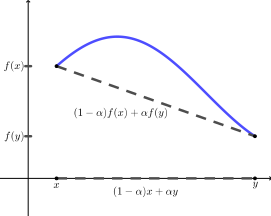
\includegraphics{Concave}}
\caption{A concave function.}
\label{F:concave}
\end{center}
\end{figure}

\ba

\item Let $f(x) = -x^2$ map $\R$ to $\R$ with the standard Euclidean metric. Show that $f$ is concave on the interval $[-1,1]$.  (Hint: Start with the fact that $\alpha(1-\alpha)(x-y)^2 \geq 0$.)

\item Show that if $f$ is a concave function on $[0,\infty)$ and $f(0) \geq 0$, an interval and $a$ and $b$ are in the interval, then 
\[f(a) + f(b) \geq f(a+b).\]
(Hint: Consider (\ref{eq:concave}) with $y=0$. Then use the fact that $\frac{a}{a+b}$ is in $[0,1]$.)

\item Suppose $(X,d)$ is a metric space and $f: [0, \infty) \to [0, \infty)$ is an increasing, concave function such that $f(x) = 0$ if and only if $x=0$. Prove that $f \circ d$ is a metric on $X$. 

\ea

\begin{comment}

\ExerciseSolution 

\ba

\item Let $x$ and $y$ be in $[-1,1]$ and let $\alpha$ be between $0$ and $1$. Since $\alpha$ and $1-\alpha$ are both between $0$ and $1$, and $(x-y)^2 \geq 0$, we have that 
\begin{align*}
\alpha(1-\alpha)(x-y)^2 &\geq 0 \\
(\alpha-\alpha^2)(x^2-2xy+y^2)  &\geq 0 \\
\alpha(x^2-2xy+y^2) - \alpha^2(x^2-2xy+y^2) &\geq 0 \\
\alpha x^2 - \alpha^2x^2 - 2 \alpha xy + 2\alpha^2xy - \alpha^2y^2 + \alpha y^2 &\geq 0 \\
 \big( -x^2 +2 \alpha x^2 - \alpha^2 x^2 -  2 \alpha xy + 2\alpha^2xy - \alpha^2y^2 \big)  + (x^2 - \alpha x^2 + \alpha y^2) &\geq 0 \\
  \big( -(1-\alpha)^2x^2 - 2\alpha(1-\alpha)xy - \alpha^2y^2 \big) + (x^2 - \alpha x^2 + \alpha y^2) &\geq 0 \\
  -((1-\alpha)x + \alpha y)^2 -((1-\alpha)(-x^2) + \alpha (-y^2)) &\geq 0 \\
f((1-\alpha)x + \alpha y) - ((1-\alpha)f(x) + \alpha f(y)) &\geq 0  \\
f((1-\alpha)x + \alpha y)  &\geq (1-\alpha)f(x) + \alpha f(y).
\end{align*}

So $f$ is concave on $[-1,1]$. Note that this argument doesn't depend on $x$ and $y$ begin in the interval $[-1,1]$, so $f$ is concave on any interval. 

\item First note that if $y=0$ we have 
\[f(tx) \geq tf(x) + (1-t) f(y) \geq tf(x)\]
for all $x \in [0,\infty)$ and all $t \in [0,1]$. 
Let $a, b \in [0, \infty)$ with $a \neq b$. Then 
\[f(a)+f(b) = f\left(\frac{a}{a+b}(a+b)\right) + f\left(\frac{b}{a+b}(a+b)\right) \geq \frac{a}{a+b}f(a+b) + \frac{a}{a+b}f(a+b) = f(a+b).\]

\item Let $x, y, z \in X$. Since the codomain of both $f$ and $d$ is the set of non-negative real numbers, we conclude that $(f \circ d)(x,y) \geq 0$. Also,
\[(f \circ d)(x,y) = f(d(x,y)) = f(d(y,x)) = (f \circ d)(y,x)\]
and $f \circ d$ is symmetric. 

Suppose $x=y$. Then 
\[(f \circ d)(x,y) = f(d(x,x)) = f(0) = 0.\]
Conversely, suppose $(f \circ d)(x,y) = 0$. Then $f(d(x,y)) = 0$. The fact that $f(t) = 0$ if and only if $t=0$ implies that $d(x,y) = 0$. Thus, $x=y$. 

Finally, we address the triangle inequality. The result of part (a) and the fact that $f$ is increasing show that  
\begin{align*}
(f \circ d)(x,y) + (f \circ d)(y,z) &= f(d(x,y)) + f(d(y,z)) \\
	&\geq f(d(x,y)+d(y,z)) \\
	&\geq f(d(x,z) \\
	&= (f \circ d)(x,z).
\end{align*}

\ea

\end{comment}



\item For each of the following, answer true if the statement is always true. If the statement is only sometimes true or never true, answer false and provide a concrete example to illustrate that the statement is false. If a statement is true, explain why. 
	\ba
	\item The function $d: \R \times \R \to \R$ defined by $d(x,y) = (x-y)^2$ is a metric on $\R$. 

	\item Every nonempty set can be made into a metric space. 
	
	\item It is possible to define an infinite number of metrics on every set containing at least two elements.

	\item Let $(X, d_X)$ and $(Y, d_Y)$ be metric spaces with $|X| \geq 2$. Then the function $d: X \times Y \to \R$ defined by $d((a,b),(c,d)) = d_X(a,c)d_Y(b,d)$ is a metric on $X \times Y$.
	
	\item Let $(X,d)$ be a metric space. If $X$ is infinite, then the range of $d$ is also an infinite set. 

			
	\ea

\begin{comment}

\ExerciseSolution

	\ba
	
	\item This statement is false. Although $d$ satisfies $d(x,y) \geq 0$ and $d(x,y) = d(y,x)$ for all $x$, $y$ in $\R$, and $d(x,y) = 0$ if and only if $x=y$, the function $d$ fails to satisfy the triangle inequality. Note that $d(1,3) = 2^2 = 4$ but 
	\[d(1,2) + d(2,3) = 1^2+1^2 = 2 < d(1,3).\]
	
		\item This statement is true. The discrete metric is a metric on any set. 
	
	\item This statement is true. If $d$ is a metric on a set $X$ and $k$ is a positive real number, then $kd : X \times X \to \R$ defined by $(kd)(x,y) = k(d(x,y))$ is also a metric. To see why, let $x$, $y$, and $z$ be in $X$
	\begin{itemize}
	\item The fact that $d(x,y) \geq 0$ implies that $kd(x,y) \geq 0$. 
	\item Since $d(x,y) = d(y,x)$ it is also the case that $kd(x,y) = kd(y,x)$.
	\item Because $d(x,x) = 0$ we also have $kd(x,x) = 0$, and if $kd(x,y) = 0$, then $d(x,y) = 0$ which makse $x = y$.
	\item Finally $kd$ satisfies the triangle inequality:
	\[(kd)(x,z) = k(d(x,z)) \leq k(d_x,y) + d(y,z)) = kd(x,y) + kd(y,z) = (kd)(x,y) + (kd)(y,z).\]
	\end{itemize}
	
	\item This statement is false. Let $x_1$ and $x_2$ be distinct elements in $X$ and let $y \in Y$. Then
	\[d((x_1,y), (x_2,y)) = d_X(x_1,x_2)d_Y(y,y) = 0\]
	even though $(x_1,y) \neq (x_2,y)$. 
		
	\item This statement is false. Let $X = \R$ with the discrete metric. Then the range of $d$ is $\{0,1\}$. 

	
	\ea


\end{comment}

\ee
